\chapter{Reinforcement learning with graph neural networks}
\label{chap:math}

Deep learning and neural networks have achieved unprecedented success since their introduction and currently being state-of-the-art in numerous fields, such as object detection \cite{DBLP:journals/corr/RedmonDGF15, 10.1109/IVS.2019.8813777, 8627998}, machine translation \cite{DBLP:journals/corr/LuongPM15, 8003957, DBLP:journals/corr/abs-2002-07526}, and many others \cite{DONG2021100379, 10.1145/3505243, PICCIALLI2021111}. Many deep learning techniques involve learning from Euclidian data (e.g., images, text, and videos). At the same time, there is an increasing number of fields where data is represented as graphs. For example, the interaction of users on social media \cite{10.1145/3308558.3313488}, atoms and their bonds in protein molecules \cite{strokach2020fast}, and traffic forecasting \cite{JIANG2022117921}. Learning from graph data has created significant challenges. Graphs can be irregular, with varying numbers of nodes, and each node can have a different number of neighbors. As a result, some important operations (e.g., convolution) can not be applied the same way as in the case of images. With growing interest in deep learning from graph data, new methods motivated by Convolutional Neural Networks (CNNs) and Recurrent Neural networks (RNNs) have been developed. For example, an image can be thought of as a graph, where each node is a pixel, and edges connect nodes partaking in convolution, as illustrated in Figure 2.1 below \cite{9046288}.\\
\begin{center}
    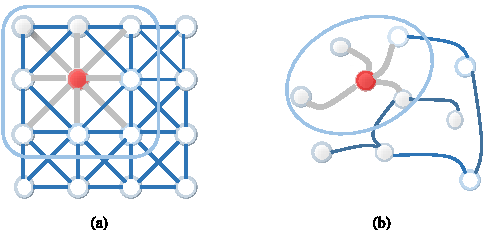
\includegraphics[width=0.6\linewidth]{images/image_vs_graph.pdf}\\
    Figure 2.1: 2-D Convolution versus graph convolution \cite{9046288}
\end{center}
